\section{Introduction}
\label{sec:intro}

World models have been widely recognized as a foundation toward general intelligence~\citep{genie3, worldlabs2025marble, xiang2025pan, ali2025world}, with a growing consensus that learning to predict the world is prerequisite to acting effectively within it~\citep{lecun2022path, hafner2023mastering, hafner2025training, assran2025v}.
\citet{richens2025general} further prove a stronger claim: any agent capable of generalizing across a sufficiently broad range of tasks must have learned a world model, establishing world models not merely as useful but as necessary for general-purpose agents.

\looseness=-1 Yet the language environments in which LLM agents operate still lack a general-purpose world model.
In the agent–environment interaction loop, two complementary components are essential: the policy~(states $\rightarrow$ actions) and the world model~((states, actions) $\rightarrow$ subsequent states).
However, current research on LLM agents has focused almost exclusively on the policy side.
We argue that world modeling is a crucial missing piece in the path to general agents.
\textbf{In this work, we explore both how to achieve language world modeling and how to apply it to advance general agents.}
We first study world modeling in language models to devlop a foundation model, the Language World Model (LWM), for agentic environment simulation.
We then investigate how world modeling can improve general agents through two complementary paradigms: either decoupling the agent from the world model or unifying them into a single framework.

\definecolor{boxbrown}{HTML}{862D1A}
\definecolor{boxwarm}{HTML}{F7F4ED}
\begin{tcolorbox}[
  enhanced,
  colback=boxwarm!30,
  colframe=boxbrown!80,
  colbacktitle=boxwarm,
  coltitle=boxbrown!90!black,
  fonttitle=\small,
  title={\textbf{Why Language World Models When Real Environments Exist?}\\{Not for Cost Reduction, but as a Complementary Axis for Pushing the Frontier}},
  boxrule=0.5pt,
  arc=1.5pt,
  left=8pt, right=8pt, top=4pt, bottom=4pt,
  toptitle=3pt, bottomtitle=3pt,
]
\textbf{(1) Decoupling:} Using the world model as a simulator facilitates turn-level scalability and controllability.
(i) Scalability:
LWM enables turn-level scaling of diverse environments without requiring dedicated infrastructure (e.g., sandboxes or GUI virtual machines), spanning extreme scenarios, real-world tasks~\citep{openclaw2026,patwardhan2025gdpval}, and high-value professional domains where real execution is infeasible due to irreversible operations, proprietary deployments, or the absence of public implementations.
(ii) Controllability:
LWM offers precise controllability, enabling more diverse and challenging environments that systematically expose agent weaknesses through targeted perturbations rare or absent in real environments.
For instance, it can return partial results that force the agent to take additional interaction steps to retrieve the complete information.
Training against these targeted perturbations helps agents handle edge cases that real-environment training alone cannot cover, ultimately surpassing agents trained solely in real environments (\S\ref{sec:app:controllable}).

\smallskip
\textbf{(2) Unifying:} A capable general agent should possess both decision-making and world-modeling abilities.
World modeling serves as a foundation for stronger agents, as it enables agents to predict future states to refine action selection, whereas traditional agent training has focused only on state-to-action decision-making.
Intuitively, an agent capable of predicting environment feedback prior to committing to an action can in principle perform no worse than its counterpart lacking such capacity~\citep{richens2025general}.
Next state prediction can thus be internalized as a meta-level thinking pattern similar to ``reflection'' but oriented toward the future (\S\ref{sec:app:foundation}).
Furthermore, accurate next-state prediction requires reasoning, knowledge, instruction following, and long-context handling (Appendix~\ref{sec:analysis:reasoning}), capabilities that are themselves foundational to general agents.
\end{tcolorbox}


We present \textbf{\method}, the first language world model that simulates seven agent environments through long chain-of-thought reasoning: MCP, Search, Terminal, Software Engineering, Android, Web, and OS.
For the three GUI domains, environment observations are represented as accessibility trees and UI view hierarchies rather than pixel frames.
\method is a \emph{native} world model trained through three stages: CPT injects state-transition dynamics and world knowledge, SFT activates next-state-prediction thinking patterns, and RL with hybrid rubric-and-rule rewards sharpens simulation fidelity.
To evaluate LWM, we construct \textbf{\bench}, a comprehensive benchmark across all seven domains.
The benchmark is built from real environment interactions of frontier models such as Claude Opus 4.6 on widely used agent benchmarks such as Terminal-Bench 1.0 \& 2.0~\citep{merrill2026terminal} and OSWorld-Verified~\citep{xie2024osworld} ensuring entirely out-of-distribution evaluation.
\bench evaluates simulation quality through open-ended rubric judging across five dimensions.
We additionally design rule-based verifiers for deterministic checks on targeted simulation capabilities.
Empirical evaluations demonstrate that \method achieves superior performance over existing frontier models.
We further investigate two complementary paradigms by which world modeling improves general agents:

\begin{itemize}[leftmargin=1.5em,itemsep=2pt,topsep=0pt]

\item \textbf{Environment Simulator~(\S\ref{sec:app:simulator}).}
We demonstrate that \method can simulate $4k$ real-world OpenClaw environments for agentic RL, yielding gains on Claw-Eval~\citep{ye2026claw} and QwenClawBench~\citep{qwenclawbench}.
Moreover, the controllability provides significant advantages complementary to real-world interaction, leading to substantial gains on Tool Decathlon~\citep{li2025tool}, MCPMark~\citep{wu2025mcpmark}, and WideSearch~\citep{wong2025widesearch}.

\item \textbf{Agent Foundation Model~(\S\ref{sec:app:foundation}).}
Comprehensive experiments on Terminal-Bench 2.0~\citep{merrill2026terminal}, SWE-Bench Verified~\citep{jimenez2024swe}, SWE-Bench Pro~\citep{deng2025swe}, BFCL~v4~\citep{patil2025berkeley}, Claw-Eval~\citep{ye2026claw}, QwenClawBench~\citep{qwenclawbench}, and WideSearch~\citep{wong2025widesearch} demonstrate that LWM training serves as a warm-up or auxiliary training stage.
It acquaints agents with environment dynamics and next-state prediction before downstream agentic RL, thereby providing a critical foundation for bootstrapping stronger agent performance.


\end{itemize}

\begin{figure}[t]
    \centering
    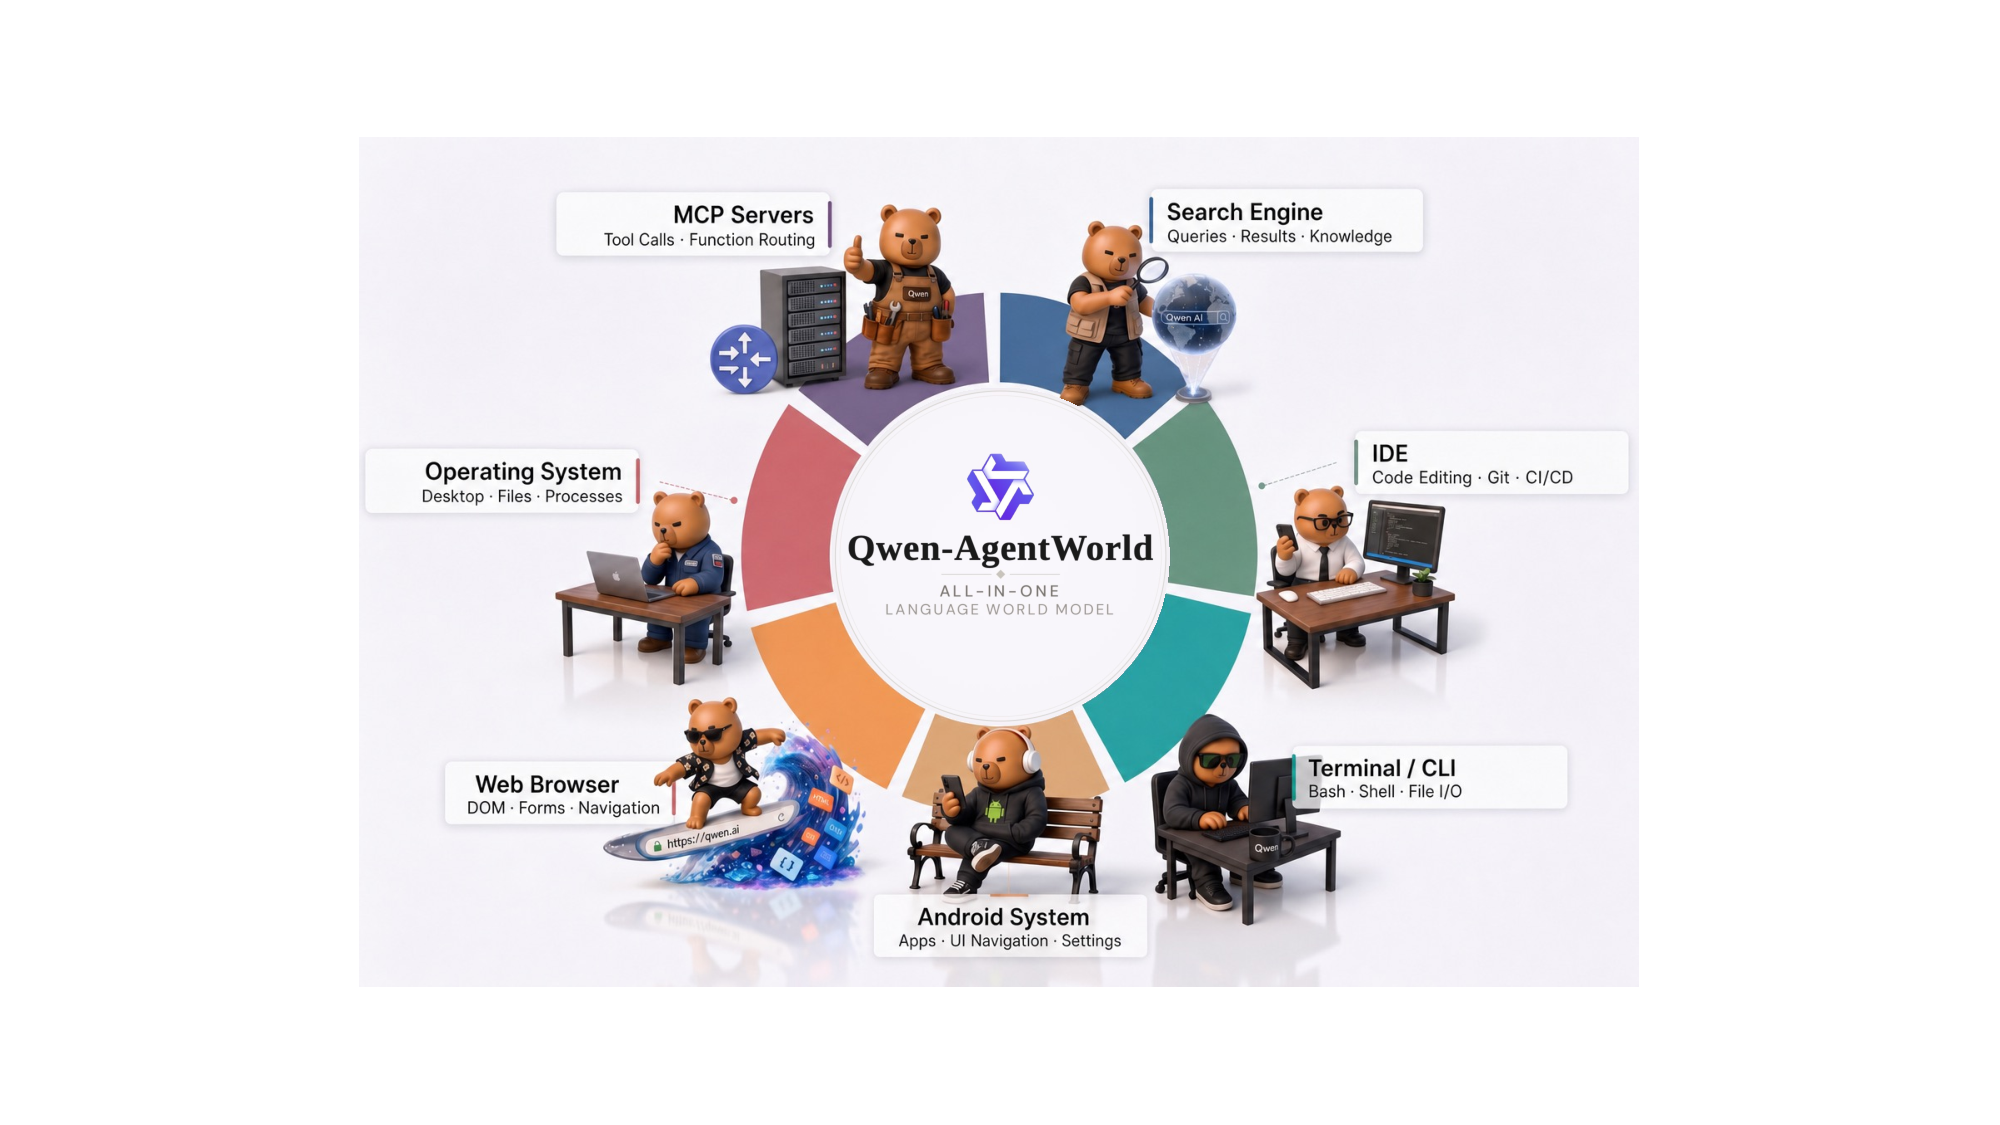
\includegraphics[width=\linewidth]{figures/group_capybaras_v2.2.pdf}
    \caption{\method unifies seven categories of interactive environment simulation within a single language world model.
    }
    \label{fig:all_in_one}
\end{figure}
